\hypertarget{gauge-degeneracy-and-the-euler-equation}{%
\subsubsection{Gauge Degeneracy and the Euler Equation}\label{gauge-degeneracy-and-the-euler-equation}}

\hypertarget{fig:state_decomposition_animated}{%
\begin{figure}
\centering
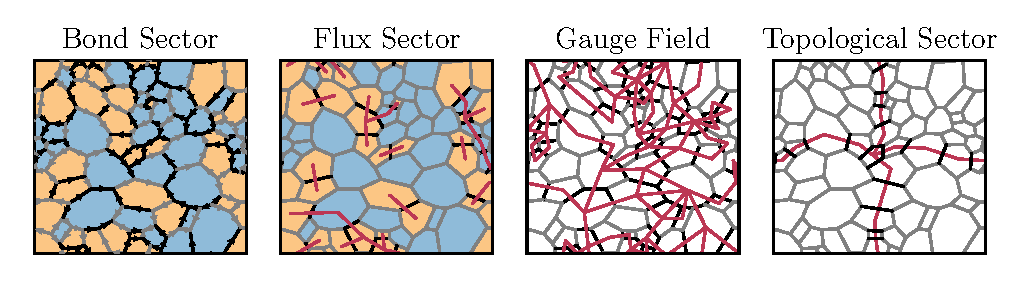
\includegraphics[width=1\textwidth,height=\textheight]{figure_code/amk_chapter/intro/state_decomposition_animated/state_decomposition_animated}
\caption[{State Decomposition}]{(Bond Sector) A state in the bond sector is specified by assigning \(\pm 1\) to each edge of the lattice. However, this description has a substantial gauge degeneracy. We can simplify things by decomposing each state into the product of three kinds of objects: (Vortex Sector) Only a small number of bonds need to be flipped (compared to some arbitrary reference) to reconstruct the vortex sector. Here, the edges are chosen from a spanning tree of the dual lattice, so there are no loops. (Gauge Field) The `loopiness' of the bond sector can be factored out. This gives a network of loops that can always be written as a product of the gauge operators \(D_j\). (Topological Sector) Finally, there are two loops that have no effect on the vortex sector, nor can they be constructed from gauge symmetries. These can be thought of as two fluxes \(\Phi_{x/y}\) that thread through the major and minor axes of the torus. Measuring \(\Phi_{x/y}\) amounts to constructing Wilson loops around the axes of the torus. We can flip the value of \(\Phi_{x}\) by transporting a vortex pair around the torus in the \(y\) direction, as shown here. In each of the three figures on the right, black bonds correspond to those that must be flipped. Composing the three together gives back the original bond sector on the left. \href{http://thomashodson.com/assets/thesis/figure_code/amk_chapter/intro/state_decomposition_animated/state_decomposition_animated.gif}{ Animated version online.}}
\label{fig:state_decomposition_animated}
\end{figure}
}

We can check this analysis with a counting argument. For a lattice with \(B\) bonds, \(P\) plaquettes and \(V\) vertices, we can count the number of bond sectors, vortices sectors and gauge symmetries and check them against Euler's polyhedra equation.

Euler's equation states for a closed surface of genus \(g\), i.e that has \(g\) holes so \(0\) for the sphere, \(1\) for the torus and \(g\) for \(g\) tori stuck together \[B = P + V + 2 - 2g\]

For the case of the torus where \(g = 1\), we can rearrange this to read: \[B = (P-1) + (V-1) + 2\]

\textbf{Bond Sectors}: Each \(u_{ij}\) takes two values and there is one associated with each bond so there are exactly \(2^B\) distinct configurations of the bond sector. Let us see if we can factor those configurations out into the Cartesian product of vortex sectors, gauge symmetries and non-contractible loop operators.

\textbf{Vortex sectors}: Each plaquette operator \(\phi_i\) takes two values (\(\pm 1\) or \(\pm i\)) and there are \(P\) of them. Vortices can only be created in pairs so there are \(\tfrac{2^P}{2} = 2^{P-1}\) vortex sectors in total. Denoting the number of pairs of vortices as \(N_v\), the vortex parity \(1 - 2*(N_v \mod 2)\) will be relevant in the projector later.

\textbf{Gauge symmetries}: As discussed earlier, these correspond to all possible compositions of the \(D_j\) operators. Again, there are only \(2^{V-1}\) of these because, as we will see in the next section, \(\prod_{j} D_j = \mathbb{1}\) in the physical space. We enforce this by choosing the correct product of single particle fermion states. One can get an intuitive picture for why \(\prod_{j} D_j = \mathbb{1}\) by imagining larger and larger patches of \(D_j\) operators on the torus. These patches correspond to transporting a vortex pair around the edge of the patch. At some point, the patch wraps around and starts to cover the entire torus. As this happens, the boundary of the patch disappears and, hence, it corresponds to the identity operation. See \cref{fig:flood_fill} and \cref{fig:flood_fill_amorphous}.

\textbf{Topological Sectors}: Finally, the torus has two non-contractible loop operators associated with its major and minor diameters. These give us two extra fluxes \(\Phi_x\) and \(\Phi_y\) each with two distinct values.

Putting this all together, we see that there are \textbf{\(2^B\) bond sectors} a space which can be decomposed into the Cartesian product of \textbf{\(2^{P-1}\) vortex sectors}, \textbf{\(2^{V-1}\) gauge symmetries} and \textbf{\(2^2 = 4\) topological sectors}.

The topological sector forms the basis of proposals to construct topologically protected qubits since the four sectors can only be mixed by a highly non-local perturbations~\autocite{kitaev_fault-tolerant_2003}.

Takeaway: The Extended Hilbert Space decomposes into a direct product of Flux Sectors, four Topological Sectors and a set of gauge symmetries.

\hypertarget{counting-edges-plaquettes-and-vertices}{%
\subsubsection{Counting edges, plaquettes and vertices}\label{counting-edges-plaquettes-and-vertices}}

It is useful to know how the trivalent structure of the lattice constrains the number of bonds \(B\), plaquettes \(P\) and vertices \(V\) it has.

The lattice is built from vertices that each share three edges with their neighbours. This means that each vertex comes with \(\tfrac{3}{2}\) bonds i.e \(3V = 2B\). This is consistent with the fact that, in the Majorana representation on the torus, each vertex brings three \(b^\alpha\) operators which then pair along bonds to give \(3/2\) bonds per vertex.

If we define an integer \(N\) such that \(V = 2N\) and \(B = 3N\) and substitute this into the polyhedra equation for the torus, we see that \(P = N\). Therefore, if a trivalent lattice on the torus has \(N\) plaquettes, it has \(2N\) vertices and \(3N\) bonds.

We can also consider the sum of the number of bonds in each plaquette \(S_p\), since each bond is a member of exactly two plaquettes \[S_p = 2B = 6N\]

The mean size of a plaquette in a trivalent lattice on the torus is exactly six. As the sum is even, this also tells us that all odd plaquettes must come in pairs.

\hypertarget{fig:flood_fill_amorphous}{%
\begin{figure}
\centering
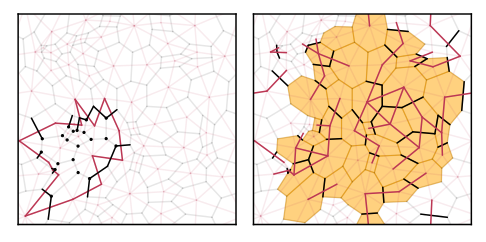
\includegraphics[width=1\textwidth,height=\textheight]{figure_code/amk_chapter/intro/flood_fill_amorphous/flood_fill_amorphous}
\caption[{Gauge Operators on Amorphous Lattices}]{The same as \cref{fig:flood_fill} but for the amorphous lattice. \href{http://thomashodson.com/assets/thesis/figure_code/amk_chapter/intro/flood_fill_amorphous/flood_fill_amorphous.gif}{ Animated version online.}}
\label{fig:flood_fill_amorphous}
\end{figure}
}

\hypertarget{quick-breather}{%
\subsubsection{Quick Breather}\label{quick-breather}}

Let's consider where are with the model now. We can map the spin Hamiltonian to a Majorana Hamiltonian in an extended Hilbert space. Along with that mapping comes a gauge field \(u_{jk}\) defining \textbf{bond sectors}. The gauge symmetries of \(u_{jk}\) are generated by the set of \(D_j\) operators. The gauge invariant, and, therefore, physically, relevant variables are the plaquette operators \(\phi_i\) which define as a \textbf{vortex sector}. To solve the Majorana Hamiltonian, we must remove hats from the gauge field by restricting ourselves to a particular bond sector. At this stage, the Majorana Hamiltonian becomes non-interacting and we can solve it like any quadratic theory. This lets us construct the single particle eigenstates from which we can also construct many body states. Yet, the many body states constructed in this way are not in the physical subspace!

For the many body states within a particular bond sector, \(\mathcal{P}_0 = 0,1\) tells us which of those overlap with the physical sector.

We see that finding a state that has overlap with a physical state only ever requires the addition or removal of one fermion. There are cases where this can make a difference, but for most observables, such as ground state energy, this correction scales away as the number of fermions in the system grows.

If we wanted to construct a full many body wavefunction in the spin basis, we would need to include the full symmetrisation over the gauge fields. However, this was not necessary for any of the results that will be presented here.

\hypertarget{the-ground-state}{%
\subsection{The Ground State}\label{the-ground-state}}

\_\_ drastically shorten to make space for discussion of generalisations\_\_

We have shown that the Hamiltonian is gauge invariant. As a result, only the flux sector and the two topological fluxes affect the spectrum of the Hamiltonian. Thus, we can label the many body ground state by a combination of fluxes and fermionic occupation numbers.

By studying the projector, we saw that the fermionic occupation numbers of the ground state will always be either \(n_m = 0\) or \(n_0 = 1, n_{m>1} = 0\) because the projector only enforces combined vortex and fermion parity.

I refer to the flux sector that contains the ground state as the ground state flux sector. Recall that the excitations of the fluxes away from the ground ground state configuration are called \textbf{vortices}, so that the ground state flux sector is, by definition, the vortex free sector.

On the Honeycomb, Lieb's theorem implies that the ground state corresponds to the state where all \(u_{jk} = 1\). This implies that the flux free sector is the ground state sector~\autocite{lieb_flux_1994}.

Lieb's theorem does not generalise easily to the amorphous case. However, we can get some intuition by examining the problem that will lead to a guess for the ground state. We will then provide numerical evidence that this guess is in fact correct.

Consider the partition function of the Majorana hamiltonian: \[ \mathcal{Z} = \mathrm{Tr}\left( e^{-\beta H}\right) = \sum_i \exp{-\beta \epsilon_i}\] At low temperatures \(\mathcal{Z} \approx \beta \epsilon_0\) where \(\epsilon_0\) is the lowest energy fermionic state.

How does the \(\mathcal{Z}\) depend on the Majorana hamiltonian? Expanding the exponential out gives \[ \mathcal{Z} = \sum_n \frac{(-\beta)^n}{n!} \mathrm{Tr(H^k)} \]

This makes for an interesting observation. The Hamiltonian is essentially a scaled adjacency matrix. An adjacency matrix being a matrix \(g_{ij}\) such that \(g_{ij} = 1\) if vertices \(i\) and \(j\) and joined by an edge and 0 otherwise.

Powers of adjacency matrices have the property that the entry \((g^n)_{ij}\) corresponds to the number of paths of length \(n\) on the graph that begin at site \(i\) and end at site \(j\). These include somewhat degenerate paths that go back on themselves.

Therefore, the trace of an adjacency matrix \[\mathrm{Tr}(g^n) = \sum_i (g^n)_{ii}\] counts the number of loops of size \(n\) that can be drawn on the graph.

Applying the same treatment to our Majorana Hamiltonian, we can interpret \(u_{ij}\) to equal 0 if the two sites are not joined by a bond and we put ourselves in the isotropic phase where \(J^\alpha = 1\) \[ \tilde{H}_{ij} =  \tfrac{1}{2} i u_{ij}\]

We then see that the trace of the nth power of H is a sum over Wilson loops of size \(n\) with an additional factor of \(2^{-n}\). We showed earlier that the Wilson loop operators can always be written as products of the plaquette operators that they enclose.

Lumping all the prefactors together, we will get something schematically like: \[ \mathcal{Z} = c_A \hat{A} + c_B \hat{B} + \sum_i c_i \hat{\phi}_i + \sum_{ij} c_{ij}  \hat{\phi}_i \hat{\phi}_j + \sum_{ijk} c_{ijk}  \hat{\phi}_i \hat{\phi}_j \hat{\phi}_k + ...\]

Where the \(c\) factors would be something like \[c_{ijk...} = \sum_n \tfrac{(-\beta)^n}{n!} \tfrac{1}{2^n} K_{ijk...}\] This is a sum over all loop lengths \(n\) with, for each, a combinatorial factor \(K_{ijk...}\) that counts how many ways exist to draw a loop of length \(n\) that only encloses plaquettes \(ijk...\).

We also have the pesky topological fluxes \(\Phi_x\) and \(\Phi_y\). Again, the prefactors for these are very complicated. However, we can intuitively see that for larger and larger loops lengths, there will be a combinatorial explosion of possible ways that they appear in these sums. We know that explosion will be suppressed exponentially for sufficiently large system sizes but for practical lattices they cause significant finite size effects.

We do not have much hope of actually evaluating this for an amorphous lattice. However, we can guess that the ground state vortex sector might be a simple function of the side length of each plaquette.

The ground state of the Amorphous Kitaev Model is found by setting the flux through each plaquette \(\phi\) to be equal to \(\phi^{\mathrm{g.s.}}(n_{\mathrm{sides}})\)

\[\begin{aligned}
    \phi^{\mathrm{g.s.}}(n_{\mathrm{sides}}) = -(\pm i)^{n_{\mathrm{sides}}},
\end{aligned}\] where \(n_{\mathrm{sides}}\) is the number of edges that form each plaquette and the choice of sign gives a twofold chiral ground state degeneracy.

This conjecture is consistent with Lieb's theorem on regular lattices~\autocite{lieb_flux_1994} and is supported by numerical evidence. As noted before, any flux that differs from the ground state is an excitation which we call a vortex.

\hypertarget{finite-size-effects}{%
\subsubsection{Finite size effects}\label{finite-size-effects}}

This guess only works for larger lattices. To rigorously test it, we would want to directly enumerate the \(2^N\) vortex sectors for a smaller lattice and check that the lowest state found is the vortex sector predicted by our conjecture.

To do this we tile an amorphous lattice as the unit cell of a periodic \(N\times N\) system. Bonds that originally crossed the periodic boundaries now connect adjacent unit cells. Using Bloch's theorem, the problem essentially reduces back to the single amorphous unit cell. However, now the edges that cross the periodic boundaries pick up a phase dependent on the crystal momentum \(\vec{q} = (q_x, q_y)\) and the lattice vector of the bond \(\vec{x} = (+1, 0, -1, +1, 0, -1)\). Assigning these lattice vectors to each bond is also a very convenient way to store and plot toroidal graphs.

This can then be solved using Bloch's theorem. For a given crystal momentum \(\textbf{q} \in [0,2\pi)^2\), we are left with a Bloch Hamiltonian, which is identical to the original Hamiltonian aside from an extra phase on edges that cross the periodic boundaries in the \(x\) and \(y\) directions, \[\begin{aligned}
    M_{jk}(\textbf{q}) =  \frac{i}{2} J^{\alpha} u_{jk} e^{i q_{jk}},\end{aligned}\] where \(q_{jk} = q_x\) for a bond that crosses the \(x\)-periodic boundary in the positive direction, with the analogous definition for \(y\)-crossing bonds. We also have \(q_{jk} = -q_{kj}\). Finally, \(q_{jk} = 0\) if the edge does not cross any boundaries at all. In essence, we are imposing twisted boundary conditions on our system. The total energy of the tiled system can be calculated by summing the energy of \(M( \textbf{q})\) for every value of \(\textbf{q}\).

With this technique, the finite size effects related to the non-contractible loop operators are removed with only a linear penalty in computation time compared to the exponential penalty paid by simply diagonalising larger lattices.

This technique verifies that \(\phi_0\) correctly predicts the ground state for hundreds of thousands of lattices with up to twenty plaquettes. For larger lattices, we verified that random perturbations around the predicted ground state never yield a lower energy state.

\hypertarget{chiral-symmetry}{%
\subsubsection{Chiral Symmetry}\label{chiral-symmetry}}

The discussion above shows that the ground state has a twofold \textbf{chiral} degeneracy which arises because the global sign of the odd plaquettes does not matter.

This happens because we have broken the time reversal symmetry of the original model by adding odd plaquettes~\autocite{Chua2011,yaoExactChiralSpin2007,ChuaPRB2011,Fiete2012,Natori2016,Wu2009,Peri2020,WangHaoranPRB2021}.

Similarly to the behaviour of the original Kitaev model in response to a magnetic field, we get two degenerate ground states of different handedness. Practically speaking, one ground state is related to the other by inverting the imaginary \(\phi\) fluxes~\autocite{yaoExactChiralSpin2007}.

\hypertarget{fig:majorana_bound_states}{%
\begin{figure}
\centering
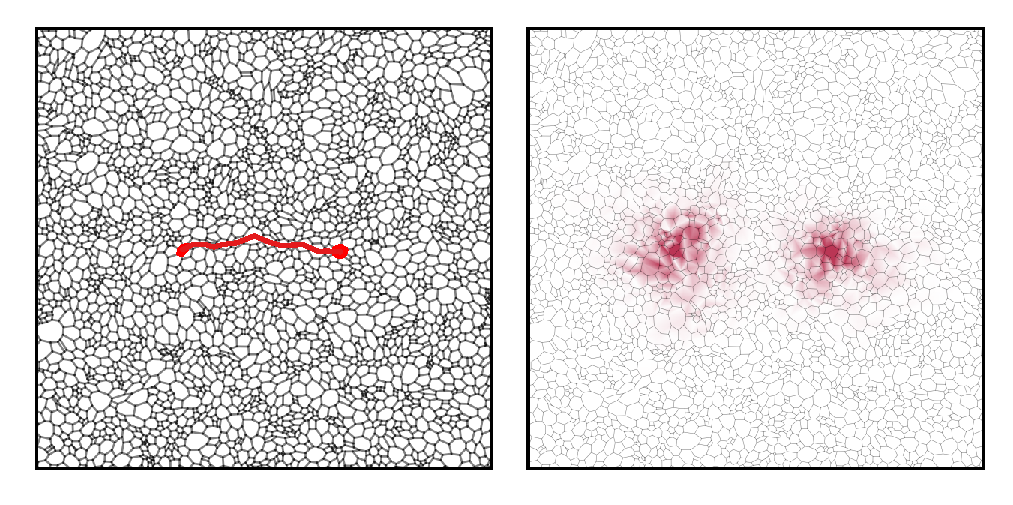
\includegraphics[width=1\textwidth,height=\textheight]{figure_code/amk_chapter/majorana_bound_states/majorana_bound_states}
\caption[{Majorana Bound States}]{(Left) A large amorphous lattice in the ground state save for a single pair of vortices shown in red, separated by the string of bonds that we flipped to create them. (Right) The density of the lowest energy Majorana state in this vortex sector. These Majorana states are bound to the vortices. They `dress' the vortices to create a composite object.}
\label{fig:majorana_bound_states}
\end{figure}
}
